\section{EL GRUPO DE LAS TRANSFORMACIONES}\label{ch:grupo}
	\subsection{Nuevas definiciones y nuevas transformaciones}
		Las f\'ormulas de las transformaciones dodecaf\'onicas quedaron de esta forma:
				
		\begin{center}
		$\mbox{I}(\sigma(m))= -\sigma(m) + 2\sigma(0)$\\
		$\mbox{T}^{\mbox{k}}(\sigma(m))=\ \sigma(m) + \mbox{k}$\\
		$\mbox{R}(\sigma(m))=\ \sigma(-1-m)$
		\end{center}
			
		Sin embargo, la importancia de estas definiciones radica en qu\'e espectro serial forman, y no en c\'omo se nombra cada serie espec\'ifica. No es distinguible a un nivel musical y, de hecho, hay m\'as de un convenio para ello.
		
		Han surgido a lo largo de la historia dos m\'etodos para nombrar las series. El primero, el m\'etodo tradicional, se ha usado desde al menos 1945. El segundo, el m\'etodo de tonos absolutos, fue concebido por George Perle en su libro \emph{Twelve Tone Tonality} (1977).
		
		En el m\'etodo tradicional, T$_0$ se usa para la primera serie que se encuentra en la composici\'on; es decir, la serie original. En cambio, el m\'etodo de tonos absolutos nombra las series T bas\'andose solamente en la nota en la que comienzan: T$_0$ se usa para la serie que comienza por un Do, y as\'i sucesivamente. En ambas, las series transpuestas se nombran como $\Psi_{\mbox{k}}$.
		
		Estas nomenclaturas no caracterizan adecuadamente el objeto matem\'atico que deben representar, es decir, funciones aplicadas a las series. Son nombres arbitrarios que adem\'as producen ambig\"uedad al a\~nadir otras funciones o al intentar describirlo matem\'aticamente.
		
		En todo caso, cualquier convenio de notaci\'on tendr\'a f\'ormulas matem\'aticas distintas al resto, pero todas preservan el material compositivo de la obra. Eso quiere decir que se pueden redefinir algunas de las transformaciones, siempre que preserven el sentido musical. 
		
		Por ejemplo, la inversi\'on puede prescindir de ser transportada para que la primera nota coincida con la original. Para distinguirla de la primera definici\'on, \'esta se llamar\'a S de simetr\'ia: $\mbox{S}(\sigma(m)) = -\sigma(m)$.
		
		E igual que la inversi\'on es el cambio de signo por fuera, la retrogradaci\'on puede convertirse simplemente en el cambio de signo por dentro. \'Esta se llamar\'a V de volteo: $\mbox{V}(\sigma(m)) = \sigma(-m)$. \footnote{Si no se a\~nade la transformaci\'on C, entonces V no conserva el espectro serial de \{I,T,R\}.}
		
		As\'i quedan dos transformaciones que se asemejan a reflexiones: una por \textit{dentro} y otra por \textit{fuera}; y una adici\'on por \textit{fuera}. Aqu\'i \textit{dentro} significa \textit{antes} de aplicar $\sigma$ y \textit{fuera} significa \textit{despu\'es} de aplicar $\sigma$, ya que no se debe olvidar que $\sigma$, la permutaci\'on, es una funci\'on en s\'i misma. Y ahora surge una cuesti\'on consecuentemente: ¿cu\'al ser\'ia entonces el resultado de sumar \textit{dentro}, es decir, \textit{antes}?
		
		Esta nueva transformaci\'on, cuya aparici\'on resulta natural tras las otras tres, se llama \textit{desplazamiento c\'iclico}. Inventada y usada por Alban Berg, y en algunas obras primerizas de Schoenberg, C$^{\mbox{k}}$ desplaza el comienzo de la serie k posiciones m\'as all\'a:
		\[\mbox{C}^{\mbox{k}}(\sigma(m))=\sigma(m+\mbox{k})\]	
			
		\[\mbox{C}^{\mbox{k}}=
		\left(\begin{array}{*{7}c}
		0&1&2&&9&10&11\\
		\sigma(\mbox{k})&\sigma(\mbox{k}+1)&\sigma(\mbox{k}+2)&\cdots&\sigma(\mbox{k}+9)&\sigma(\mbox{k}+10)&\sigma(\mbox{k}+11)\\
		\end{array}\right)\]
		
		La serie 4-c\'iclica sobre la permutaci\'on P de la Suite Op. 25 es la siguiente serie C$^4$:	
		\[\mbox{C}^4=\drow{6,3,8,2,11,0,9,10,4,5,7,1}\]		
		\begin{center}
			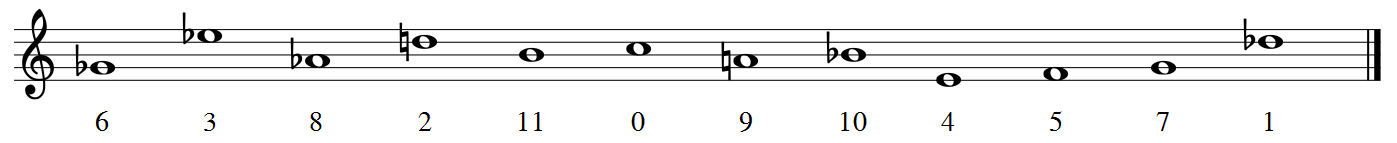
\includegraphics[width=12.1cm]{13.png}
		\end{center}
				
		En resumen, se puede trabajar con un nuevo sistema de definiciones que mantienen el significado musical del serialismo pero var\'ian la notaci\'on con la que se trabaja. 
		
		\begin{multicols}{2}
		\begin{align*}
		\mbox{S}(\sigma(m)) &= -\sigma(m)\\
		\mbox{T}^{\mbox{k}}(\sigma(m)) &= \sigma(m) + \mbox{k}
		\end{align*}
		
		\begin{align*}
		\mbox{V}(\sigma(m)) &= \sigma(-m)\\
		\mbox{C}^{\mbox{k}}(\sigma(m)) &= \sigma(m+\mbox{k})
		\end{align*}
		\end{multicols}
	
	\subsection{Diagramas de reloj}
	
		Para visualizar mejor c\'omo act\'uan las distintas transformaciones, las series se pueden representar mediante \textit{diagramas de reloj}: una sucesi\'on de aristas con una orientaci\'on establecida que conecta los v\'ertices de un dodec\'agono en el orden de la serie \cite{hunter}. Ya que el desplazamiento c\'iclico act\'ua como si la serie fuese circular, hay a\~nadida una arista desde la \'ultima nota a la primera. El comienzo de la serie y su orientaci\'on se marcan con una flecha.
		
		\begin{figure}[h]
			\begin{center}				
			\ddiagram{4,5,7,1,6,3,8,2,11,0,9,10}{T$^0$}
			\end{center}
		\end{figure} 
		
		Arriba se incluye el diagrama de la serie original $\sigma$ de la Suite Op. 25. Se pueden distinguir las caracter\'isticas de la serie, como las tres diagonales, que son los tres intervalos de tritono. A continuaci\'on se incluyen los diagramas de las transformaciones dodecaf\'onicas originales: la transposici\'on, la inversi\'on y la retrogradaci\'on; as\'i como el nuevo desplazamiento c\'iclico.
		
	\begin{center}
		\begin{multicols}{4}
		\ddiagram[4]{5,6,8,2,7,4,9,3,0,1,10,11}{T$^1$}
		\ddiagram[4]{10,9,0,11,2,8,3,6,1,7,5,4}{R}
		\ddiagram{4,3,1,7,2,5,0,6,9,8,11,10}{I}
		\ddiagram[4]{5,7,1,6,3,8,2,11,0,9,10,4}{C$^1$}
	\end{multicols}
	\end{center}
		
		La transposici\'on es una rotaci\'on en el sentido en el que apunta la flecha; la inversi\'on es una reflexi\'on con el eje de simetr\'ia en la diagonal que pasa por la flecha; la retrogradaci\'on es un cambio de orientaci\'on de la flecha; y el desplazamiento c\'iclico es el avance interno de la flecha por el recorrido de la serie.		
		
		La diferencia entre las inversiones I y S es precisamente la transposici\'on de $2\sigma(0)=8$ semitonos en este ejemplo. Comparando S con T$^0$ se puede adem\'as observar que S es una reflexi\'on con el eje de simetr\'ia en 0, en vez de que el eje dependa de la propia permutaci\'on.
		
		\begin{center}
			\begin{multicols}{2}				
				\ddiagram{4,3,1,7,2,5,0,6,9,8,11,10}{I}				
				
				\ddiagram[4]{8,7,5,11,6,9,4,10,1,0,3,2}{S}
			\end{multicols}
		\end{center}
	
		Por otro lado, la comparaci\'on entre las retrogradaciones R y V muestra que, aunque en principio m\'as arbitraria, V es una transformaci\'on m\'as natural, ya que deja fija la flecha. La diferencia entre ellas es en realidad un desplazamiento c\'iclico de -1.
		
		\begin{center}
			\begin{multicols}{2}
				\ddiagram[4]{10,9,0,11,2,8,3,6,1,7,5,4}{R}				
				
				\ddiagram{4,10,9,0,11,2,8,3,6,1,7,5}{V}
			\end{multicols}
		\end{center}

		He creado una p\'agina interactiva que genera diagramas de reloj de cualquier serie para cualquier longitud serial, adem\'as de generar series aleatorias. Tambi\'en se pueden aplicar las transformaciones a la serie, tanto las originales como las del nuevo sistema, para ver c\'omo se comporta el diagrama. Est\'a escrita en Elm y el c\'odigo puede encontrarse en \url{https://gitlab.com/dodecafonismo/diagramas}.
	
		En el enlace \url{https://diagramas.netlify.com} se accede a la aplicaci\'on web. Sus instrucciones de uso se encuentran al final de la p\'agina.
		
		Adem\'as, he creado un comando en \LaTeX{} que dibuja estos diagramas dada su serie y su nombre, as\'i como el n\'umero que est\'a arriba: \verb|\ddiagram[4]{4,5,7,1,6,3,8,2,11,0,9,10}{T$^0$}| -- en este caso \verb|[4]| no es necesario, ya que por defecto se coloca arriba la primera nota de la serie. El c\'odigo se encuentra en el enlace \url{https://gitlab.com/dodecafonismo/ddphonism}.
	
	\subsection[El grupo: D$_{12}$ x D$_{12}$]{El grupo: D$_{\textbf{12}}$ x D$_{\textbf{12}}$}
		El conjunto de transformaciones \{S, T, V, C\} est\'a compuesto por dos parejas con semejanzas entre s\'i. S es una reflexi\'on y T una rotaci\'on de orden 12 -- es decir, que al aplicarla 12 veces se vuelve a la identidad -- y ambas se aplican a la figura entera; es como mover el diagrama por el papel. En cambio, V es una reflexi\'on de la flecha en s\'i, y C una rotaci\'on -- tambi\'en de orden 12 -- de la flecha sobre la l\'inea; ambas aplicadas al interior de la figura.
		
		Cada pareja genera un grupo muy conocido: el grupo di\'edrico o diedral. Se denota\footnote{En otros \'ambitos, D$_n$ tambi\'en se denota por D$_{2n}$, ya que $2*n$ es el n\'umero de elementos que tiene el grupo.} por D$_{12}$ y representa el grupo de simetr\'ias de un pol\'igono regular; en este caso, un dodec\'agono. Por ejemplo, aqu\'i se muestran todas las simetr\'ias de un oct\'ogono, que son los 16 elementos de D$_{8}$, aplicados a una se\~nal de STOP.
		
		\begin{center}
		\begin{tikzpicture}[scale=1.8]
		\foreach \i in {0,...,7}
		\node[regular polygon,regular polygon sides=8,draw,rotate=-45*\i] at (\i,1) {STOP};
		\foreach \i in {0,...,7}
		\node[regular polygon,regular polygon sides=8,draw,rotate=-45*\i,xscale=-1] at (\i,0) {STOP};		
		\end{tikzpicture}
		\end{center}
	
		De igual manera, el conjunto de series de un espectro serial se consigue aplicando a la serie las distintas funciones transformativas; se obtiene entonces un grupo di\'edrico para ambas parejas de funciones. 
		
		Al haber dos parejas distintas que act\'uan por separado dentro y fuera de la figura, el grupo completo que forman las cuatro transformaciones es el producto directo de dos copias del di\'edrico: D$_{12}\times\mbox{D}_{12}$.
		
		Podemos observarlo claramente si representamos la serie de una segunda forma: como la correspondencia entre v\'ertices de dos dodec\'agonos. La serie original, que es en realidad una permutaci\'on de 12 elementos, se representa como una funci\'on: los v\'ertices del dodec\'agono interno se env\'ian biyectivamente a los v\'ertices externos. As\'i, $m \longmapsto \sigma(m)$. Este diagrama es similar al matricial pero enroscado en s\'i mismo, de tal forma que se aprecia la permutaci\'on escogida mediante las flechas, que son fijas, y facilita un significado del antes y el despu\'es de aplicarla.
		
		Las dos primeras figuras describen esto mismo: la representaci\'on de la serie original y la representaci\'on de la permutaci\'on mediante las flechas, que se mantendr\'an constantes en el resto de figuras.
			\begin{center}
				\begin{multicols}{2}
				\begin{tikzpicture}
				\ddihedral{4,5,7,1,6,3,8,2,11,0,9,10}
				\end{tikzpicture}
				
				\begin{tikzpicture}
				\darrows{4,5,7,1,6,3,8,2,11,0,9,10}
				\end{tikzpicture}
			\end{multicols}
			\end{center}
	
		Las cuatro siguientes figuras representan las cuatro funciones transformativas, que son en realidad la reflexi\'on y la rotaci\'on del grupo di\'edrico de cada dodec\'agono. Aplicarlo al de dentro es aplicarlo antes de las flechas; antes de la permutaci\'on. Aplicarlo fuera es transformar despu\'es de las flechas; despu\'es de la permutaci\'on.
		
		\begin{center}
			\begin{multicols}{2}
			
\begin{tikzpicture}
			\ddihedral[s=1]{4,5,7,1,6,3,8,2,11,0,9,10}
			\draw [very thick,dash pattern={on 1pt off 4pt on 10pt off 3pt}] (0,-3.5) -- (0,-0.5);
			\draw [very thick,dash pattern={on 1pt off 4pt on 10pt off 3pt}] (0,0.5) -- (0,3.5);
			\end{tikzpicture}
			
			\begin{tikzpicture}
			\ddihedral[t=1]{4,5,7,1,6,3,8,2,11,0,9,10}			
			\draw [style=rotateArrow,thick,dashed] (90:3) to [bend right=45] (180:3);
			\node at (0,3.25) {};
			\end{tikzpicture}
		\end{multicols}
		
		\begin{multicols}{2}
			\begin{tikzpicture}
			\ddihedral[v=1]{4,5,7,1,6,3,8,2,11,0,9,10}			
			\draw [very thick,dash pattern={on 1pt off 3pt on 7pt off 2pt}] (0,-2) -- (0,-0.5);
			\draw [very thick,dash pattern={on 1pt off 3pt on 7pt off 2pt}] (0,0.5) -- (0,2);
			\end{tikzpicture}
			
			\begin{tikzpicture}
			\ddihedral[c=1]{4,5,7,1,6,3,8,2,11,0,9,10}			
			\draw [style=rotateArrow,thick,dashed] (90:1.75) to [bend left=45] (0:1.75);
			\end{tikzpicture}
		\end{multicols}
		\end{center}
	
	He creado un comando en \LaTeX{} que dibuja estos diagramas di\'edricos dada su serie original y las funciones aplicadas a ella: \verb|t|, \verb|s|, \verb|c| y \verb|v|. Se aplican en ese mismo orden, y por defecto est\'an a 0. \linebreak \verb|\ddihedral[c=2,t=3,s=1]{4,5,7,1,6,3,8,2,11,0,9,10}|. El c\'odigo se encuentra en el enlace \url{https://gitlab.com/dodecafonismo/ddphonism}.
	
	\subsection{Conmutatividad entre los elementos del grupo}		
		La rotaci\'on (r) y la reflexi\'on (s) de un grupo di\'edrico no conmutan, sino que cumplen $r\cdot s=s\cdot r^{-1}$. Por otro lado, en los productos directos los elementos de un lado conmutan con los del otro. As\'i, \{S, T\} y \{V, C\} no conmutan, pero el resto de parejas s\'i. La verificaci\'on de estas afirmaciones, que confirman que el grupo generado es D$_{12}\times\mbox{D}_{12}$, se encuentran %en el Anexo \ref{app:commm}.
		a continuaci\'on:
			\begin{center}
			\begin{multicols}{3}
				\ \linebreak
				
				\begin{align*}
				&\ \text{S}\circ\text{T}(\sigma(m))\\
				=&\ \text{S}(\sigma(m)+1)\\
				=&\ -(\sigma(m)+1)\\
				=&\ -\sigma(m)-1
				\end{align*}
				
				\underline{S y T no conmutan:}
				
				\begin{align*}
				&\ \text{T}\circ\text{S}(\sigma(m))\\
				=&\ \text{T}(-\sigma(m))\\
				=&\ -\sigma(m)+1
				\end{align*}			
				
				\ \linebreak
				
				\begin{align*}
				&\ \text{S}\circ\text{T}^{-1}(\sigma(m))\\
				=&\ \text{S}(\sigma(m)-1)\\
				=&\ -(\sigma(m)-1)\\
				=&\ -\sigma(m)+1
				%=&\ \text{T}\circ\text{S}(\sigma(m))
				\end{align*}
			\end{multicols}
			
			\begin{multicols}{3}
				\ \linebreak
				
				\begin{align*}
				&\ \text{V}\circ\text{C}(\sigma(m))\\
				=&\ \text{V}(\sigma(m+1))\\
				=&\ \sigma(-(m+1))\\
				=&\ \sigma(-m-1)
				\end{align*}
				
				\underline{V y C no conmutan:}
				
				\begin{align*}
				&\ \text{C}\circ\text{V}(\sigma(m))\\
				=&\ \text{C}(\sigma(-m))\\
				=&\ \sigma(-m+1)
				\end{align*}
				
				\ \linebreak
				
				\begin{align*}
				&\ \text{V}\circ\text{C}^{-1}(\sigma(m))\\
				=&\ \text{V}(\sigma(m-1))\\
				=&\ \sigma(-(m-1))\\
				=&\ \sigma(-m+1)
				%=&\ \text{C}\circ\text{V}(\sigma(m))
				\end{align*}
			\end{multicols}
			
			\begin{multicols}{3}
				\begin{align*}
				&\ \text{S}\circ\text{V}(\sigma(m))\\
				=&\ \text{S}(\sigma(-m))\\
				=&\ -\sigma(-m)
				\end{align*}
				
				\underline{S y V conmutan:}
				
				\begin{align*}
				&\ \text{V}\circ\text{S}(\sigma(m))\\
				=&\ \text{V}(-\sigma(m))\\
				=&\ -\sigma(-m)
				\end{align*}
			\end{multicols}
			
			\begin{multicols}{3}
				\begin{align*}
				&\ \text{S}\circ\text{C}(\sigma(m))\\
				=&\ \text{S}(\sigma(m+1))\\
				=&\ -\sigma(m+1)
				\end{align*}
				
				\underline{S y C conmutan:}
				
				\begin{align*}
				&\ \text{C}\circ\text{S}(\sigma(m))\\
				=&\ \text{C}(-\sigma(m))\\
				=&\ -\sigma(m+1)
				\end{align*}
			\end{multicols}
			
			\begin{multicols}{3}
				\begin{align*}
				&\ \text{T}\circ\text{V}(\sigma(m))\\
				=&\ \text{T}(\sigma(-m))\\
				=&\ \sigma(-m)+1
				\end{align*}
				
				\underline{T y V conmutan:}
				
				\begin{align*}
				&\ \text{V}\circ\text{T}(\sigma(m))\\
				=&\ \text{V}(\sigma(m)+1)\\
				=&\ \sigma(-m)+1
				\end{align*}
			\end{multicols}
			
			\begin{multicols}{3}
				\begin{align*}
				&\ \text{T}\circ\text{C}(\sigma(m))\\
				=&\ \text{T}(\sigma(m+1))\\
				=&\ \sigma(m+1)+1
				\end{align*}
				
				\underline{T y C conmutan:}
				
				\begin{align*}
				&\ \text{C}\circ\text{T}(\sigma(m))\\
				=&\ \text{V}(\sigma(m)+1)\\
				=&\ \sigma(m+1)+1
				\end{align*}
			\end{multicols}
		\end{center}
		
		Volviendo a las definiciones originales \{I, T, R, C\}, su estructura interna es bien distinta. El problema de I es que depende de la permutaci\'on escogida, por lo que a veces tiene unas propiedades y a veces otras. En cambio, la definici\'on de V con respecto a R es meramente est\'etica: ya que no depende de la permutaci\'on, su conmutatividad se mantiene invariante. 
		
		Viendo c\'omo conmutan los elementos de este sistema se aprecia la dificultad de I. Curiosamente, la conmutatividad de \{I, R\} e \{I, C\} se pierde, pero se gana la de \{I, T\}. As\'i, T conmuta con todo en el sistema. Esto muestra una ventaja de la definici\'on de I.
		
		\begin{multicols}{3}
			\begin{align*}
		&\ \mbox{I}\circ\mbox{R}(\sigma(m))\\
		=&\ \mbox{I}(\mbox{R}(\sigma(m)))\\
		=&\ -\mbox{R}(\sigma(m))+2\mbox{R}(\sigma(0))\\
		=&\ -\sigma(-1-m)+2\sigma(-1-0)\\
		=&\ -\sigma(-1-m)+2\sigma(-1)
		\end{align*}
		
		\underline{I y R ya no conmutan:}
		
		\begin{align*}
		&\ \mbox{R}\circ\mbox{I}(\sigma(m))\\
		=&\ \mbox{R}(\mbox{I}(\sigma(m)))\\
		=&\ \mbox{R}(-\sigma(m)+2\sigma(0))\\
		=&\ \mbox{R}(-\sigma(m))+2\sigma(0)\\
		=&\ -\sigma(-1-m)+2\sigma(0)
		\end{align*}
		\end{multicols}
		
		Los \'unicos casos en los que podr\'ian conmutar ocurrir\'ian cuando
		\begin{align*}
		2\sigma(0)\equiv2\sigma(-1)\ \mbox{(mod. 12)}&\impliedby\\
		12+2\sigma(0)=2\sigma(-1)&\Longleftrightarrow\\
		6+\sigma(0)=\sigma(-1)&\Longleftrightarrow\\
		\sigma(-1)-\sigma(0)=6&
		\end{align*}
		
		Es decir, cuando la primera y la \'ultima nota de la serie original se distancian en 6 semitonos, como es el caso de la permutaci\'on en la Suite Op. 25:
		
		\[
		\mbox{IR}=\mbox{RI}=\drow{10,11,8,9,6,0,5,2,7,1,3,4}
		\]	
		
		\begin{center}
		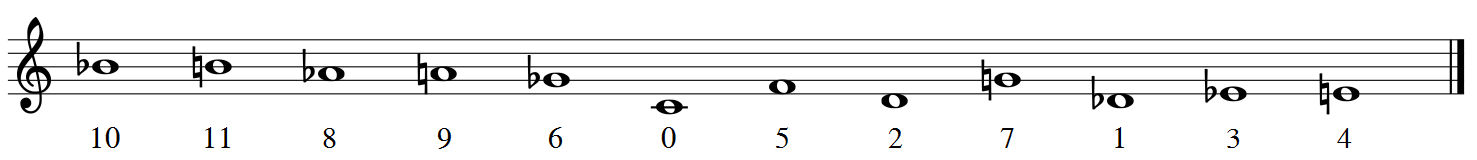
\includegraphics[width=12.1cm]{5.png}
		\end{center}
		
		\begin{multicols}{3}
			\begin{align*}
			&\ \mbox{I}\circ\mbox{C}(\sigma(m))\\
			=&\ \mbox{I}(\sigma(m+1))\\
			=&\ -\sigma(m+1)+2\sigma(1)
			\end{align*}
			
			\underline{I y C ya no conmutan:}
			
			\begin{align*}
			&\ \mbox{C}\circ\mbox{I}(\sigma(m))\\
			=&\ \mbox{C}(-\sigma(m)+2\sigma(0))\\
			=&\ \mbox{C}(-\sigma(m))+2\sigma(0)\\
			=&\ -\sigma(m+1)+2\sigma(0)
			\end{align*}
		\end{multicols}
		
		Los \'unicos casos en los que podr\'ian conmutar son cuando
		\begin{align*}
		2\sigma(0)\equiv2\sigma(1)\ \mbox{(mod. 12)}&\impliedby\\
		12+2\sigma(0)=2\sigma(1)&\Longleftrightarrow\\
		6+\sigma(0)=\sigma(1)&\Longleftrightarrow\\
		\sigma(1)-\sigma(0)=6&
		\end{align*}
		
		Es decir, cuando la primera y la segunda nota de la serie original se distancian en 6 semitonos.
		
		Si se echan las cuentas con C$^{\mbox{k}}$ en vez de con C$^1$, pueden conmutar si $\sigma(\mbox{k})-\sigma(0)=6$. Como $\sigma$ es una permutaci\'on, devuelve todos los valores de 0 a 11 y solamente una vez cada uno. Por tanto, tambi\'en devuelve 6 + $\sigma(0)$, as\'i que \textbf{siempre existe un \'unico k para el que I y C$^{\mbox{k}}$ conmutan}. En el caso de la permutaci\'on de la Suite Op. 25, como $\sigma(0)=4$ hay que encontrar el k para el que $\sigma(\mbox{k})=4+6=10$. En este caso, $\mbox{k}=11$, pero depende por completo de la permutaci\'on original.\\
		
		\begin{multicols}{3}
			\begin{align*}
			&\ \mbox{I}\circ\mbox{T}(\sigma(m))\\
			=&\ \mbox{I}(\sigma(m)+1)\\
			=&\ -(\sigma(m)+1) + 2(\sigma(0)+1)\\
			=&\ -\sigma(m)-1+2\sigma(0)+2\\
			=&\ -\sigma(m)+2\sigma(0)+1
			\end{align*}
			
			\underline{I y T ahora s\'i conmutan:}\\
			
			\begin{align*}
			&\ \mbox{T}\circ\mbox{I}(\sigma(m))\\
			=&\ \mbox{T}(-\sigma(m)+2\sigma(0))\\
			=&\ -\sigma(m)+2\sigma(0)+1
			\end{align*}
		\end{multicols}
		
		\begin{multicols}{3}
		\begin{align*}
		&\ \mbox{R}\circ\mbox{C}(\sigma(m))\\
		=&\ \mbox{R}(\sigma(m+1))\\
		=&\ \sigma(-(m+1)-1)\\
		=&\ \sigma(-m-2)
		\end{align*}
		
		\underline{R y C no conmutan:}
		
		\begin{align*}
		&\ \mbox{C}\circ\mbox{R}(\sigma(m))\\
		=&\ \mbox{C}(\sigma(-m-1))\\
		=&\ \sigma(-m-1+1)\\
		=&\ \sigma(-m)
		\end{align*}
		\end{multicols}
		
		\begin{multicols}{3}
			\begin{align*}
			&\ \mbox{T}\circ\mbox{R}(\sigma(m))\\
			=&\ \mbox{T}(\sigma(-m-1))\\
			=&\ \sigma(-m-1)+1
			\end{align*}
			
			\underline{T y R conmutan:}
			
			\begin{align*}
			&\ \mbox{R}\circ\mbox{T}(\sigma(m))\\
			=&\ \mbox{R}(\sigma(m)+1)\\
			=&\ \sigma(-m-1)+1
			\end{align*}
		\end{multicols}
	
		\begin{multicols}{3}
			\begin{align*}
			&\ \mbox{T}\circ\mbox{C}(\sigma(m))\\
			=&\ \mbox{T}(\sigma(m+1))\\
			=&\ \sigma(m+1)+1
			\end{align*}
			
			\underline{T y C conmutan:}
			
			\begin{align*}
			&\ \mbox{C}\circ\mbox{T}(\sigma(m))\\
			=&\ \mbox{V}(\sigma(m)+1)\\
			=&\ \sigma(m+1)+1
			\end{align*}
		\end{multicols}